% Gemini theme
% https://github.com/anishathalye/gemini

\documentclass[final]{beamer}

% ====================
% Packages
% ====================

\usepackage[T1]{fontenc}
\usepackage{lmodern}
\usepackage[size=custom,width=102,height=72,scale=1.0]{beamerposter}
\usetheme{gemini}
\usecolortheme{mit}
\usepackage{graphicx}
\usepackage{booktabs}
\usepackage{tikz}
\usetikzlibrary{arrows.meta,positioning}
\usepackage{pgfplots}
\pgfplotsset{compat=1.14}
\usepackage{anyfontsize}

% ====================
% Lengths
% ====================

% If you have N columns, choose \sepwidth and \colwidth such that
% (N+1)*\sepwidth + N*\colwidth = \paperwidth
\newlength{\sepwidth}
\newlength{\colwidth}
\setlength{\sepwidth}{0.025\paperwidth}
\setlength{\colwidth}{0.30\paperwidth}

\newcommand{\separatorcolumn}{\begin{column}{\sepwidth}\end{column}}

% ====================
% Title
% ====================

\title{\huge Cyclic Polytopes and Higher Auslander Algebras}

\author{Adam Klepáč \and Jan Šťovíček}

\institute[shortinst]{Charles University in Prague}

% ====================
% Footer (optional)
% ====================

\footercontent{
  \hfill
  Groups \& Algebras in Bicocca for Young algebraists 2024 \hfill
  \href{mailto:djklepy@gmail.com}{djklepy@gmail.com}}
% (can be left out to remove footer)

% ====================
% Logo (optional)
% ====================

% use this to include logos on the left and/or right side of the header:
% \logoright{\includegraphics[height=7cm]{logo1.pdf}}
\logoleft{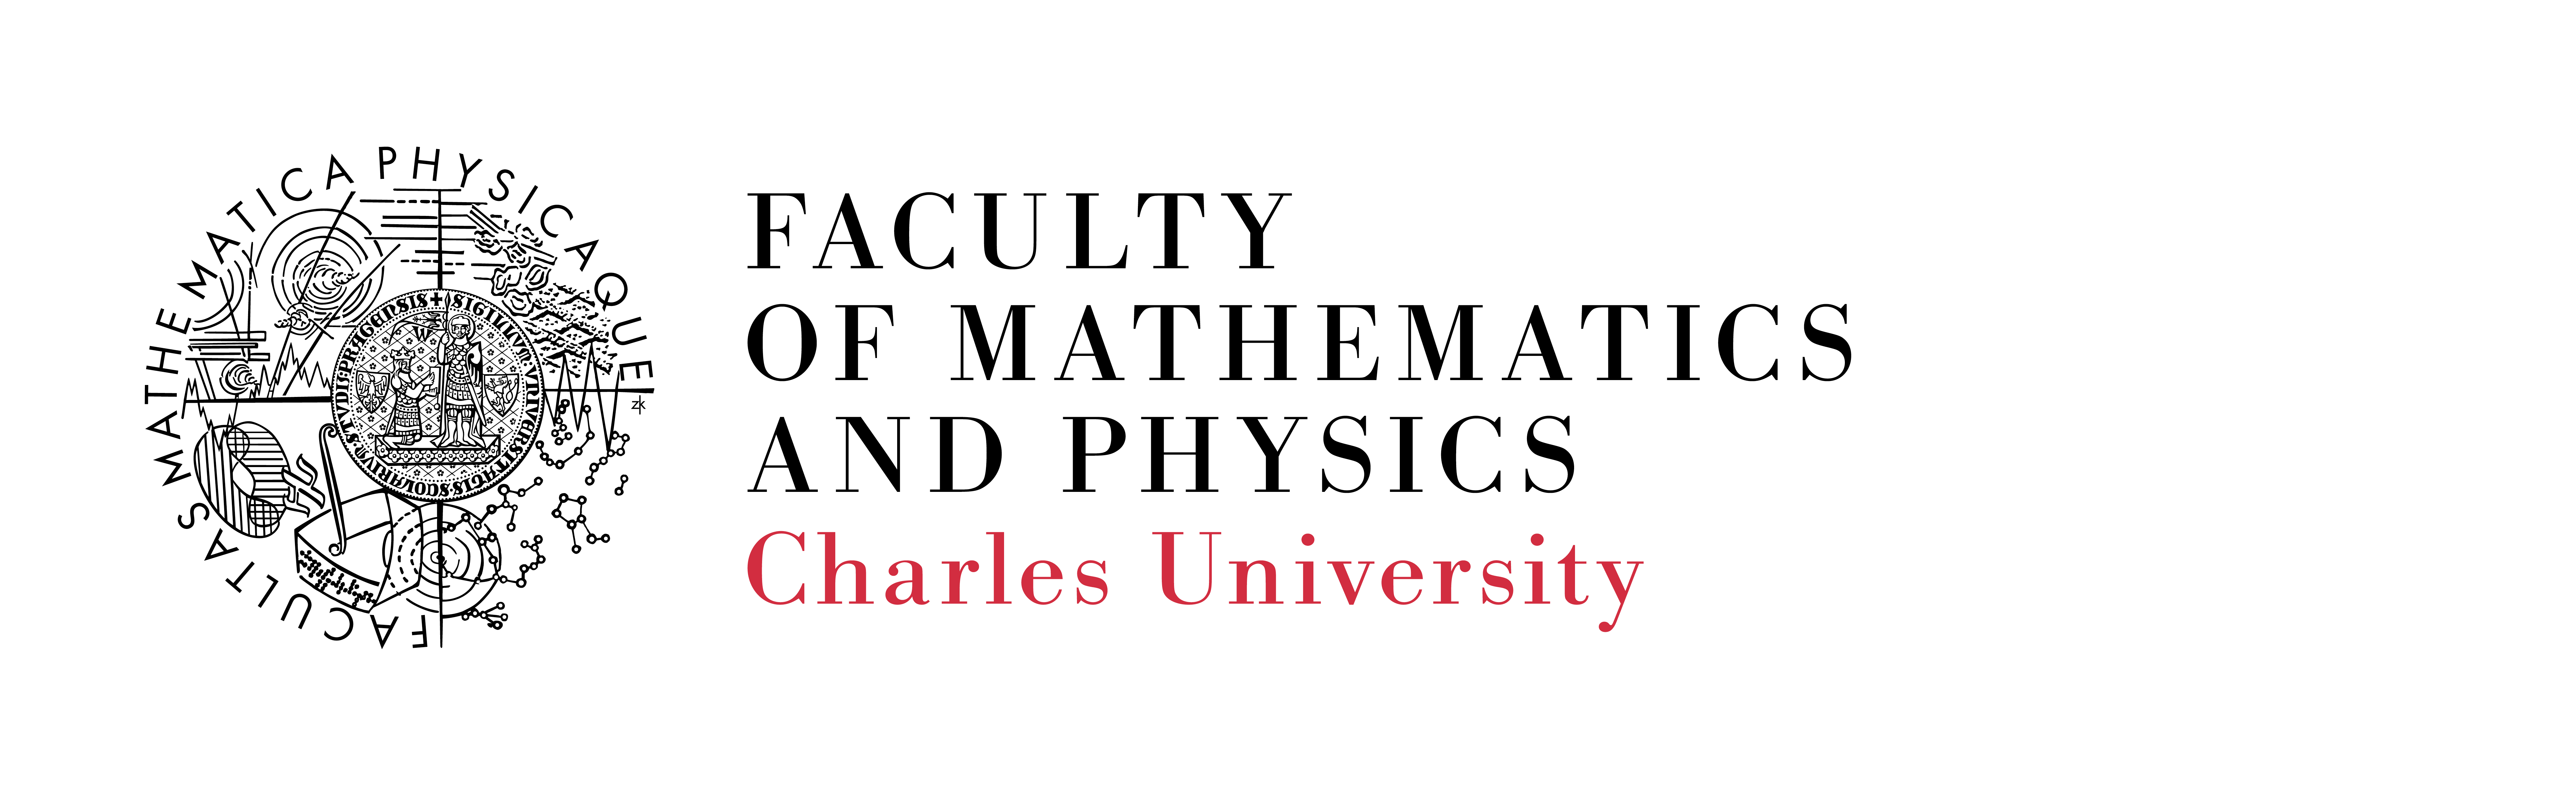
\includegraphics[height=7cm]{logo.png}}

% ====================
% Body
% ====================

\begin{document}

\begin{frame}[t]
\begin{columns}[t]
\separatorcolumn

\begin{column}{\colwidth}
  \begin{block}{Background in Representation Theory}
    \heading{Fundamental notions}
    \begin{itemize}
     \vspace*{-12pt}
     \item A \textbf{$k$-algebra} (over a field $k$) is a $k$-vector space
       equipped with a bilinear product.
     \item A \textbf{right module} over a $k$-algebra $\Lambda$ is a $k$-vector
       space with the additional operation of multiplication by elements of
       $\Lambda$ from the right which satisfies natural compatibility
       conditions.
     \item A right $\Lambda$-module $M$ is \textbf{indecomposable} if $M \neq 0$
       and $M = M_1 \oplus M_2$ implies that either of $M_1,M_2$ is zero.
     \item A \textbf{morphism} $M \to N$ of right $\Lambda$-modules is a
       $k$-linear map which respects the multiplication by elements of
       $\Lambda$.
     \item A morphism $f$ is \textbf{irreducible} if it's not invertible (from
       the left or right) and whenever it decomposes as $f = f_1 f_2$, then
       $f_1$ is invertible from the left or $f_2$ from the right.
     \item A \textbf{path algebra} of a quiver $Q$ (an oriented graph with
       multiple edges and loops) is the $k$-algebra $kQ$ with basis formed by
       all paths in $Q$ and multiplication given by concatenation.
    \end{itemize}

    \heading{Auslander-Reiten quiver}
    We can represent the category $\bmod \; \Lambda$ of right $\Lambda$-modules
    as a quiver  by considering (isomorphisms classes of) indecomposable
    $\Lambda$-modules as vertices and, informally speaking, the irreducible
    morphisms (up to a linear combination) as arrows.

    \begin{figure}[h]
     \centering
     \begin{tikzpicture}[scale=1.5]
       \node[circle,fill,inner sep=3pt] (a) at (0,0) {};
       \node[circle,fill,inner sep=3pt] (b) at (1,1) {};
       \node[circle,fill,inner sep=3pt] (c) at (2,2) {};
       \node[circle,fill,inner sep=3pt] (d) at (2,0) {};
       \node[circle,fill,inner sep=3pt] (e) at (3,1) {};
       \node[circle,fill,inner sep=3pt] (f) at (4,0) {};
       
       \draw[-{Latex[width=3mm]},thick,shorten <=2pt,shorten >=2pt] (a) -- (b);
       \draw[-{Latex[width=3mm]},thick,shorten <=2pt,shorten >=2pt] (b) -- (c);
       \draw[-{Latex[width=3mm]},thick,shorten <=2pt,shorten >=2pt] (b) -- (d);
       \draw[-{Latex[width=3mm]},thick,shorten <=2pt,shorten >=2pt] (c) -- (e);
       \draw[-{Latex[width=3mm]},thick,shorten <=2pt,shorten >=2pt] (d) -- (e);
       \draw[-{Latex[width=3mm]},thick,shorten <=2pt,shorten >=2pt] (e) -- (f);
     \end{tikzpicture}
     \caption{The Auslander-Reiten quiver of the path algebra $k($%
      \tikz[scale=1.5,baseline=-7pt]{%
        \node[circle,fill,inner sep=3pt] (a) at (0,0) {};
        \node[circle,fill,inner sep=3pt] (b) at (1,0) {};
        \node[circle,fill,inner sep=3pt] (c) at (2,0) {};
        \draw[-{Latex[width=3mm]},thick,shorten <=2pt,shorten >=2pt] (b) -- (a);
        \draw[-{Latex[width=3mm]},thick,shorten <=2pt,shorten >=2pt] (c) -- (b);
      }). This algebra has 6 indecomposable modules up to isomorphism.}
     \label{fig:ar-quiver-of-kA3}
    \end{figure}
  \end{block}

  \begin{block}{Representation-finite Hereditary Algebras}
    Every (basic connected) $k$-algebra $\Lambda$ is isomorphic to the quotient
    path algebra $kQ / I$ for some quiver $Q$ and an ideal $I$ of $kQ$.
    \begin{itemize}
      \vspace*{-12pt}
      \item The algebra $\Lambda$ is \textbf{hereditary} if every submodule of a
        projective module is itself projective.
      \item The algebra $\Lambda$ is \textbf{representation-finite} if it has
        only finitely many indecomposable modules up to isomorphism.
    \end{itemize}
    If $\Lambda$ is hereditary, then it is isomorphic directly to some path
    algebra $kQ$. If it is in addition representation-finite, then $Q$ has no
    loops or multiple edges and $Q$ (as an undirected graph) is one of
    \textbf{Dynkin} graphs (depicted in Figure~\ref{fig:dynkin-graphs}).
    \begin{figure}[h]
     \centering
      \begin{tikzpicture}[scale=1.5]
       \begin{scope}
        \node at (-1,0) {$A_n$};
        \node[circle,fill,inner sep=3pt] (a) at (0,0) {};
        \node[circle,fill,inner sep=3pt] (b) at (1,0) {};
        \node[circle,fill,inner sep=3pt] (c) at (2,0) {};
        \node (dots) at (3,0) {$\cdots$};
        \node[circle,fill,inner sep=3pt] (d) at (4,0) {};
        \node[circle,fill,inner sep=3pt] (e) at (5,0) {};

        \draw[thick] (a) -- (b);
        \draw[thick] (b) -- (c);
        \draw[thick] (c) -- (2.5,0);
        \draw[thick] (3.5,0) -- (d);
        \draw[thick] (d) -- (e);
        
       \end{scope}
       \begin{scope}[yshift=-2cm]
        \node at (-1,0) {$D_n$};
        \node[circle,fill,inner sep=3pt] (a) at (0,0) {};
        \node[circle,fill,inner sep=3pt] (b) at (1,0) {};
        \node[circle,fill,inner sep=3pt] (c) at (2,0) {};
        \node (dots) at (3,0) {$\cdots$};
        \node[circle,fill,inner sep=3pt] (d) at (4,0) {};
        \node[circle,fill,inner sep=3pt] (e) at (5,1) {};
        \node[circle,fill,inner sep=3pt] (f) at (5,-1) {};

        \draw[thick] (a) -- (b);
        \draw[thick] (b) -- (c);
        \draw[thick] (c) -- (2.5,0);
        \draw[thick] (3.5,0) -- (d);
        \draw[thick] (d) -- (e);
        \draw[thick] (d) -- (f);
       \end{scope}
       \begin{scope}[xshift=8cm]
        \node at (-1,0) {$E_6$};
        \node[circle,fill,inner sep=3pt] (a) at (0,0) {};
        \node[circle,fill,inner sep=3pt] (b) at (1,0) {};
        \node[circle,fill,inner sep=3pt] (c) at (2,0) {};
        \node[circle,fill,inner sep=3pt] (d) at (3,0) {};
        \node[circle,fill,inner sep=3pt] (e) at (4,0) {};
        \node[circle,fill,inner sep=3pt] (f) at (2,0.5) {};

        \draw[thick] (a) -- (b);
        \draw[thick] (b) -- (c);
        \draw[thick] (c) -- (f);
        \draw[thick] (c) -- (d);
        \draw[thick] (d) -- (e);
       \end{scope}
       \begin{scope}[xshift=8cm,yshift=-1.5cm]
        \node at (-1,0) {$E_7$};
        \node[circle,fill,inner sep=3pt] (a) at (0,0) {};
        \node[circle,fill,inner sep=3pt] (b) at (1,0) {};
        \node[circle,fill,inner sep=3pt] (c) at (2,0) {};
        \node[circle,fill,inner sep=3pt] (d) at (3,0) {};
        \node[circle,fill,inner sep=3pt] (e) at (4,0) {};
        \node[circle,fill,inner sep=3pt] (g) at (5,0) {};
        \node[circle,fill,inner sep=3pt] (f) at (2,0.5) {};

        \draw[thick] (a) -- (b);
        \draw[thick] (b) -- (c);
        \draw[thick] (c) -- (f);
        \draw[thick] (c) -- (d);
        \draw[thick] (d) -- (e);
        \draw[thick] (e) -- (g);
       \end{scope}
       \begin{scope}[xshift=8cm,yshift=-3cm]
        \node at (-1,0) {$E_8$};
        \node[circle,fill,inner sep=3pt] (a) at (0,0) {};
        \node[circle,fill,inner sep=3pt] (b) at (1,0) {};
        \node[circle,fill,inner sep=3pt] (c) at (2,0) {};
        \node[circle,fill,inner sep=3pt] (d) at (3,0) {};
        \node[circle,fill,inner sep=3pt] (e) at (4,0) {};
        \node[circle,fill,inner sep=3pt] (g) at (5,0) {};
        \node[circle,fill,inner sep=3pt] (h) at (6,0) {};
        \node[circle,fill,inner sep=3pt] (f) at (2,0.5) {};

        \draw[thick] (a) -- (b);
        \draw[thick] (b) -- (c);
        \draw[thick] (c) -- (f);
        \draw[thick] (c) -- (d);
        \draw[thick] (d) -- (e);
        \draw[thick] (e) -- (g);
        \draw[thick] (g) -- (h);
       \end{scope}
      \end{tikzpicture}
     \caption{All the Dynkin graphs. The number $n$ in $A_n, D_n$ and $E_n$
     denotes the number of vertices.}
     \label{fig:dynkin-graphs}
    \end{figure}
  \end{block}
\end{column}

\separatorcolumn

\begin{column}{\colwidth}
  \begin{block}{Tilting Modules \& Higher Auslander Algebras}
    A \textbf{$d$-fold extension} of a $\Lambda$-module $M$ by $N$, is an exact
    sequence
    \[
     0 \longrightarrow M \longrightarrow X_d \longrightarrow X_{d-1}
     \longrightarrow \cdots \longrightarrow X_1 \longrightarrow N
     \longrightarrow 0,
    \]
    where $X_i$ are $\Lambda$-modules. The $d$-fold extensions of $M$ by $N$
    form a group, which we denote $\mathrm{Ext}^{d}_{\Lambda}(M,N)$.

    In a representation-finite hereditary algebra $\Lambda$, a module $M$
    \begin{itemize}
     \vspace*{-12pt}
     \item is \textbf{tilting} if $\mathrm{Ext}^{1}_{\Lambda}(M,M) = 0$ and the
     number direct summands of $M$ equals the number of simple
     $\Lambda$-modules.
     \item is \textbf{$d$-cluster tilting} if
      \[
       \mathrm{add} \, M = \{X \in \bmod \, \Lambda \mid
       \mathrm{Ext}^{i}_{\Lambda}(M,X) = 0 \; \forall i \in \{1,\ldots,d-1\}\},
      \]
      where $\mathrm{add} \, M$ denotes the category of direct summands of
      direct copies of $M$.
    \end{itemize}

    The \textbf{tilting theorem}~\cite[Theorem 3.8, Chapter VI]{modraknizka}
    establishes a strong connection between the categories $\bmod \, \Lambda$
    and $\bmod \, \mathrm{End}_{\Lambda}(M)$ where $M$ is a \textbf{tilting}
    $\Lambda$-module. In case $\Lambda$ is hereditary,
    $\mathrm{End}_{\Lambda}(M)$ is a so-called \textbf{tilted algebra}, an
    important object of study in contemporary representation theory.

    The \textbf{global dimension} of $\Lambda$ is the minimal length of a
    projective resolution across all $\Lambda$-modules. Iyama~\cite{iyama}
    describes an iterative construction of $d$-representation-finite algebras
    (algebras of global dimension $ \leq d$ admitting a $d$-cluster tilting
    module). It goes like this.
    \begin{enumerate}
     \item Start with a representation-finite hereditary (also called
       $1$-representation-finite) algebra $\Lambda = \Lambda^{(1)}$. This
       algebra has a $1$-cluster tilting module $M = M^{(1)}$. Set
       $\Lambda^{(2)} = \mathrm{End}_{\Lambda}(M)$.
     \item The algebra $\Lambda^{(2)}$ is $2$-representation-finite with a
       $2$-cluster tilting module $M^{(2)}$. Set $\Lambda^{(3)} =
       \mathrm{End}_{\Lambda^{(2)}}(M^{(2)})$.
     \item[k.] The algebra $\Lambda^{(k)}$ is $k$-representation-finite with a
       $k$-cluster tilting module $M^{(k)}$. Set $\Lambda^{(k + 1)} =
       \mathrm{End}_{\Lambda^{(k)}}(M^{(k)})$. We call $\Lambda^{(k)}$ the
       \textbf{$k$-Auslander algebra} of $\Lambda$.
   \end{enumerate}
  \end{block}

  \begin{exampleblock}{Higher Auslander Algebras of Type A \& Cyclic Polytopes}
    A \textbf{cyclic polytope} $C(m,d)$ is the convex hull of a set of $m$
    points on the moment curve $t \mapsto (t, t^2, \ldots, t^{d})$ in
    $\mathbb{R}^{d}$. A \textbf{triangulation} of $C(m,d)$ is its division into
    $d$-dimensional simplices which share vertices with it.

    In~\cite{ot}, Oppermann and Thomas uncover an intriguing
    \textbf{correspondence}
    \[
     \{\text{triangulations of } C(n+2d,2d)\} \longleftrightarrow
     \{\text{tilting modules over } \Lambda^{(d)} \},
    \]
    where $\Lambda = kA_n$ (the path algebra of a linearly ordered quiver of
    Dynkin type $A$, see Figure~\ref{fig:dynkin-graphs}).
    \begin{figure}[ht]
     \centering
     \begin{tikzpicture}[scale=1.5]
      \begin{scope}
       \node[circle,fill=mitred,inner sep=4pt] (a) at (0,0) {};
       \node[circle,fill,inner sep=3pt] (b) at (1,1) {};
       \node[circle,fill=mitred,inner sep=4pt] (c) at (2,2) {};
       \node[circle,fill,inner sep=3pt] (d) at (2,0) {};
       \node[circle,fill,inner sep=3pt] (e) at (3,1) {};
       \node[circle,fill=mitred,inner sep=4pt] (f) at (4,0) {};
       
       \draw[-{Latex[width=3mm]},thick,shorten <=2pt,shorten >=2pt] (a) -- (b);
       \draw[-{Latex[width=3mm]},thick,shorten <=2pt,shorten >=2pt] (b) -- (c);
       \draw[-{Latex[width=3mm]},thick,shorten <=2pt,shorten >=2pt] (b) -- (d);
       \draw[-{Latex[width=3mm]},thick,shorten <=2pt,shorten >=2pt] (c) -- (e);
       \draw[-{Latex[width=3mm]},thick,shorten <=2pt,shorten >=2pt] (d) -- (e);
       \draw[-{Latex[width=3mm]},thick,shorten <=2pt,shorten >=2pt] (e) -- (f);
      \end{scope}
      \begin{scope}[xshift=8cm]
       \node[circle,fill,inner sep=3pt] (a) at (0,0) {};
       \node[circle,fill,inner sep=3pt] (b) at (1.2,0.1) {};
       \node[circle,fill,inner sep=3pt] (c) at (2.3,0.8) {};
       \node[circle,fill,inner sep=3pt] (d) at (3.2,1.8) {};
       \node[circle,fill,inner sep=3pt] (e) at (3.5,3) {};
       
       \draw (a) -- (b);
       \draw (b) -- (c);
       \draw (c) -- (d);
       \draw (d) -- (e);
       
       \draw[ultra thick,mitred] (a) -- (c);
       \draw[ultra thick,mitred] (c) -- (e);
       \draw[ultra thick,mitred] (a) -- (e);
      \end{scope}
     \end{tikzpicture}
     \caption{The direct sum of the \textcolor{mitred}{\textbf{coloured three
     modules}} in the Auslander-Reiten quiver of $kA_3$ is a tilting module
     corresponding to the \textcolor{mitred}{\textbf{depicted triangulation}} of
     (an illustrative version of) $C(5,2)$.}
     \label{fig:cyclic-ka3}
    \end{figure}
  \end{exampleblock}
\end{column}

\separatorcolumn

\begin{column}{\colwidth}
 \begin{alertblock}{Higher Auslander Algebras of Type D}
  We currently work on expanding this correspondence to higher Auslander
  algebras of $kD_n$ -- the path algebras of \textbf{Dynkin quivers of type D}
  (see Figure~\ref{fig:dynkin-graphs}).
  \begin{itemize}
   \vspace*{-12pt}
   \item There's an isomorphism $kD_n \cong kA_{2(n-1) - 1} / I$ for an adequate
    orientation of $A_n$ and $D_n$ and an adequate ideal $I$ (see
    Figure~\ref{fig:D4-A5}).
   \item Using this isomorphism we can partially translate the problem of
    describing tilting modules of higher Auslander algebras of type D back to
    the already understood type A.
   \item It is beneficial to view $kA_{2(n-1) - 1}$ as two linearly oriented
    $kA_{n-1}$'s. This way, we can find a correspondence between triangulations
    of two cyclic polytopes (while identifying certain pairs of simplices)
    and tilting modules of higher Auslander algebras of type D.
  \end{itemize}
  \begin{figure}[ht]
   \centering
   \begin{tikzpicture}[scale=2]
    \begin{scope}
     \node[circle,fill,inner sep=3pt] (a) at (0,0) {};
     \node[circle,fill,inner sep=3pt] (b) at (1,0) {};
     \node[circle,fill=mitred,inner sep=4pt] (c) at (2,0) {};
     \node[circle,fill,inner sep=3pt] (d) at (3,0) {};
     \node[circle,fill,inner sep=3pt] (e) at (4,0) {};

     \draw[-{Latex[width=3mm]},thick,shorten <=2pt,shorten >=2pt] (a) -- (b);
     \draw[-{Latex[width=3mm]},thick,shorten <=2pt,shorten >=2pt] (b) -- (c);
     \draw[-{Latex[width=3mm]},thick,shorten <=2pt,shorten >=2pt] (d) -- (c);
     \draw[-{Latex[width=3mm]},thick,shorten <=2pt,shorten >=2pt] (e) -- (d);

     \draw[<->,dashed,ultra thick,shorten <=2pt,shorten >=2pt] (d) to [bend left=45] (b);
     \draw[<->,dashed,ultra thick,shorten <=2pt,shorten >=2pt] (d) to [bend
      right=45] (b);
    \end{scope}
    \begin{scope}[xshift=8cm]
     \node[circle,fill=mitred,inner sep=4pt] (a) at (0,0) {};
     \node[circle,fill,inner sep=3pt] (b) at (1,0) {};
     \node[circle,fill,inner sep=3pt] (c) at (2,0.5) {};
     \node[circle,fill,inner sep=3pt] (d) at (2,-0.5) {};

     \draw[-{Latex[width=3mm]},thick,shorten <=2pt,shorten >=2pt] (b) -- (a);
     \draw[-{Latex[width=3mm]},thick,shorten <=2pt,shorten >=2pt] (c) -- (b);
     \draw[-{Latex[width=3mm]},thick,shorten <=2pt,shorten >=2pt] (d) -- (b);
    \end{scope}
   \end{tikzpicture}
   \caption{Illustration of the isomorphism $kD_4 \cong kA_5 / I$. We basically
    orient $A_5$ toward the central vertex and `glue' the paths that start at the
    same distance from the central vertex but not at the farthest vertices.}
   \label{fig:D4-A5}
  \end{figure}
 \end{alertblock}
  \begin{block}{Further Research Goals}
   \begin{itemize}
    \item Expand the described correspondence to \textbf{higher cluster
     categories} of type D (as is done for type A in~\cite[Section 6]{ot}).
    \item Focus on path algebras of \textbf{affine Dynkin quivers}, which are no
     longer representation-finite, but are close enough so that a generalized
     notion of a higher Auslander algebra is plausible.
    \item Generalize the construction of a cluster category from~\cite[Section
     5]{ot} to also include path algebras not necessarily representation-finite.
    \item Devise a \textbf{combinatorial framework} which would describe tilting modules
     over such `generalized' higher Auslander algebras and tilting objects of
     the corresponding cluster categories.
   \end{itemize}
  \end{block}

  \begin{block}{References}

    \nocite{*}
    \footnotesize{\bibliographystyle{plain}\bibliography{poster}}

  \end{block}

\end{column}

\separatorcolumn
\end{columns}
\end{frame}

\end{document}
